\documentclass[12pt,a4paper,onecolumn]{article}
\usepackage[T1]{fontenc}

\usepackage{lmodern}

%packages
\usepackage[utf8]{inputenc}
\usepackage{xcolor,graphicx}
\usepackage[a4paper,left=2.0cm,top=2.0cm,bottom=2.0cm,right=2.0cm]{geometry}
\usepackage{amsmath,amssymb} 
\usepackage[backend=biber,style=apa,sorting=nyt]{biblatex}
\usepackage{graphicx}
%reference list
\addbibresource{references.bib}

%theorem environment
\newtheorem{theorem}{Theorem}

% Define the title, author and date of the document.
\title{Forecasting GB system Inertia: An Explainable Deep Learning Analysis of Renewable Generation Impacts}
\author{Muhammad Faisal Chughtai\\
ID: 250129234}
\date{}

\begin{document}

\maketitle



\section{Introduction}
\label{sec:intro}
Great Britain's (GB) Initiative to decarbonize its energy system leads to unprecedented challenges. As the Grid transitions toward asynchronous renewable energy (solar and wind) from the traditional synchronous energy source (coal and gas), this transition is causing a critical decline in system inertia. In a power grid station, inertia mitigates the rapid changes in frequency. Moreover, insufficient inertia with minor faults leads to a high Rate of Change in Frequency (RoCoF), which increases the risk of cascading blackouts (\cite{he2024analysis}).

The National Energy System Operator (NESO) heavily relies on procuring balancing services and using conservative planning assumptions to manage risk (\cite{NESO2025Inertia}). While recent studies suggest high accuracy (\cite{dey2025system}) in ML/AI models, they can predict the inertia cost. However, these models are opaque and often operate in a black box. The control room operators, who are responsible for national energy security, are hesitant ({\cite{machlev2022explainable}}) to trust AI/ML models' predictions.

This research proposes a novel methodology that integrates SHAP with deep-learning-based inertia forecasting models. Deep learning models like Bidirectional Long Short-Term Memory (Bi-LSTM) are often seen as opaque or black-box systems. However, SHAP (Shapley Additive Explanations) integration makes these models interpretable. This methodology predicts and provides transparent insights into the factors influencing system inertia.

This study contributes to the field of applied AI by integrating XAI into power grid systems, which have previously been used to address frequency deviations ({\cite{kruse2021revealing}}). This study specifically focused on inertia forecasting. This research directly evaluates the performance of Bi-LSTM against established regression-based models and utilizes SHAP to interpret the time-series data. This addressed the key limitations and shortcomings in the literature (\cite{santosh2024inertia}).

Currently, NESCO is investing heavily in balancing services, and this study helps them reduce balancing costs through XAI integration. XAI helps operators to trust the system and make well-informed decisions (\cite{dey2025system}).

The study helps decarbonize GB energy systems by maintaining low inertia, resulting in safe grid operations (\cite{NESO2025Inertia}). This approach helps to generate more renewable energy and aligns with the UK's net-zero target.


\section{Problem Statement}
\label{sec:statement}
Unlike the European interconnected grid system, the UK’s power grid is an island system, which automatically makes it vulnerable to low-inertia events. Currently proposed methodologies rely on regional extrapolation to estimate system inertia or “Balck Box” AI models, which focus on statistical accuracy (RMSE) rather than interpretability (\cite{abouyehia2025evaluating}) to forecast system inertia.

Nesco is not fully leveraging AI models to efficiently handle low-inertia periods due to a lack of interpretability. This builds a lack of trust in operators because they are unable to verify why AI predicts a crash in inertia, and they keep running the expensive traditional fossil-fuel plant to prevent cascading blackouts. This research study focuses on both high operational accuracy and explanatory forecasting, enabling NESCO to make safety-critical, well-informed decisions. 


\section{Research Questions}
\label{sec:hypotheses}
The primary goal of this research is to bridge the gap between predictive operational accuracy and trust.

\subsection{Primary Question:}
How can XAI (SHAP) enhanced deep learning/ensemble methods outperform traditional black-box methods in forecasting GB power grid system inertia, and what meaningful insights could they provide about how the mixture of renewable energy, such as wind and solar, affects the grid stability?

\subsection{Sub-Questions:}
\begin{itemize}
\item Does Bi-LSTM guarantee better predictive operational accuracy as compared to standard LSTM and XGBoost models?
\item Is SHAP accurate enough to quantify how different renewable energy sources, specifically wind and solar, affect system inertia?
\item How does the temporal limitation of traditional SHAP (\cite{calero2025chronoshap}) affect the interpretation of time series energy data? Can window-based feature engineering improve the interpretability?
\end{itemize}


\section{Methods}
\label{sec:methods}
This research employs a quantitative, experimental approach, using historical and operationally relevant data from the NESCO data portal. The project is divided into three different phases: \textbf{Data Pre-Processing}, \textbf{Predictive Modelling}, and \textbf{Interpretation Analysis}.

\subsection{Data Pre-Processing} 
This research will use two main datasets from NESCO spanning the period from 2017 to 2025.

Firstly, this study will utilise System Inertia as the Target Variable (Y). This dataset includes the inertia measure in Gigavolt-ampere (GVAs) and is available at a 30-minute settlement period. Secondly, Historic Generation Mix will be utilised as the Predictive Modelling (X). This dataset includes categorised outputs for multiple fuel types, including wind, solar, nuclear, and Biomass. Both datasets will be treated as a single dataset and aligned by time. Moreover, the main reason for merging these two datasets is to prevent AI models from making random guesses during exceptional or unexpected weather conditions. Furthermore, if we only utilise the System Inertia dataset, this will force AI models to forecast system inertia solely based on time, leading to random guesses.

Feature Engineering will play a critical role in this research, as the dataset includes both positive contributors to system inertia, such as Nuclear and GAS, and negative contributors (\cite{he2024analysis}), such as solar and wind. Feature engineering will help separate both synchronous and asynchronous energy generation sources.

Data Cleaning will include handling missing observations via linear interpolation and normalization using a min-max scaler to efficiently handle numerical stability.

\subsection{Predictive Modelling}
To address the forecasting system's inertia, a Bi-LSTM will be developed based on recent benchmark studies (\cite{santosh2024inertia}). Bi-LSTMs are chosen as the core predictive model because they can learn temporal dependencies in both forward and backward directions. This will help to identify the underlying trends in weather-dependent data.

To validate whether deep learning is effective, two baseline approaches, the naive statistical model (ARIMA) and the widely implemented Machine Learning model (XGBoost), will be evaluated against the Bi-LSTM. This evaluation helps us to identify whether extra added complexity actually improves forecasting accuracy.

Moreover, a model evaluation will be performed using Root Mean Squared Error (RMSE) and Mean Absolute Error (MAE). RMSE is essential under low-inertia conditions; it penalizes large prediction errors, whereas MAE calculates a robust average of the forecasting accuracy between predicted and actual values.
\subsection{Interpretability Analysis}
To enable transparency, SHAP (Shapley Additive Explanations) will be implemented alongside the best-performing forecasting model, using the established KernelSHAP approach (\cite{kruse2021revealing}) to quantify each input feature's importance to the model's prediction.

Moreover, this study will address the shortcomings of applying SHAP to time-series data, specifically violations of feature independence (cited in \cite{calero2025chronoshap}). To ensure reliability, this study will focus on a “windowed” explanation approach to observe changes in feature importance over a dynamic time horizon, for example, morning peaks vs. evening demand vs. overnight demand. This way, we can ensure SHAP's reliability.


\section{Ethical Implications}
\label{sec:ethics}
This study primarily uses publicly available, non-personal datasets. Therefore, it does not involve any human participants and poses no risk to data privacy (GDPR).

However, this study focuses on the application of AI in national infrastructure, raising concerns about Automation Bias and AI safety. This study is aligned with the AI4People framework and directly supports the principle of Explicability (intelligibility and accountability). This research prevents the risk of Automation Bias by replacing “Black Box” with XAI, which reduces the risk of accepting incorrect AI predictions. Moreover, the SHAP implementations help the operator to audit the model's logic before making any critical decision. This way, control remains in the human hand, which ensures accountability.


\section{Requirements and Feasibility}
\label{sec:req}
\subsection{Requirements:}
\subsubsection{Functional Requirements:}
Implementation of a robust Python-based data pipeline for merging the “System Inertia” and "Generation Mix" datasets, as both datasets are available at 30-minute settlement periods, and a direct inner join on “Settlement Date” and "DATETIME" can easily create the required feature set.

A predictive modelling framework based on the training and evaluation of three different forecasting approaches, such as a statistical ARIMA model, a tree-based XGBoost model, and a deep learning Bi-LSTM model.

Visualisation analysis using SHAP provides transparency by providing “Summary Plots” and “Force Plots”. “Summary Plots” capture feature importance, and “Force Plots” explain the individual prediction made by the predictive modelling framework.
\subsubsection{Non-Functional Requirements}
The implemented deep-learning based approach must be reproducible and optimised to train on the standard Google Colab T4 GPU without a paid subscription.

The model can perform prediction and explanation in the minimum time possible, ensuring it's suitable for deployment in a control room environment.

\subsection{Feasibility Argument}
\textbf{Technical Feasibility:} This research is technically feasible as it relies on open-source libraries and frameworks such as scikit-learn, SPAP, TensorFlow, Keras, PyShark, and Google Colab. No paid subscription to any library or API is required to implement this project.

\textbf{Data Compatibility:} A thorough feasibility check was conducted for the target variable (System Inertia) and the input feature (Generation Mix). Both datasets have the same 30-minute settlement interval. This compatibility indicates that complex temporal resampling or interpolation is not required.

This study is based on a well-established model (\cite{dey2025system}), which significantly reduces the time required for model selection. Moreover, both datasets are perfectly aligned and highly compatible, which helps to compress the data engineering phase. Furthermore, this project highly focuses on “Analysis” rather than developing a ready-to-deploy tool. These factors combined will reduce the significant amount of time and help complete the project within the MSc Dissertation timeframe.

\subsection{Risk Management}
The major risk of Bi-LSTM is that it fails to learn the underlying pattern in time-series data (underfitting) or shows poor generalization performance (overfitting), leading to lower accuracy than other baselines. The Bi-LSTM performance evaluation is scheduled for Week 6, if XGBoost somehow outperforms the complex Bi-LSTM model. The project will change its focus from deep learning to XGBoost for SHAP analysis. As the primary objective of this research is Explainability, which can also be achieved using XGBoost.

SHAP analysis on the entire test set is computationally heavy, which can cause the “Out of Memory” Error. To mitigate this, DeepExplainer would be preferred instead of using KernelSHAP to minimize computational load.

The dataset might contain outliers or a UCT/BST time shift, which leads to poor model training and generalization performance. To mitigate this, strict UTC conversion and verification of time-based data alignment will be enforced through the data pipeline.

\section{Project Plan}
This research study strictly follows the 12-week life-cycle plan detailed in Figure \ref{fig:my_gantt_chart}, starting from data ingestion to dissertation submission. Each task in the plan is designed to be as realistic as possible.
\label{sec:proj_plan}
\begin{figure}[h]
        \centering
        % 'page=1' selects the 1st page of the PDF.
        % 'width=0.8\textwidth' scales it to 80% of the text width.
        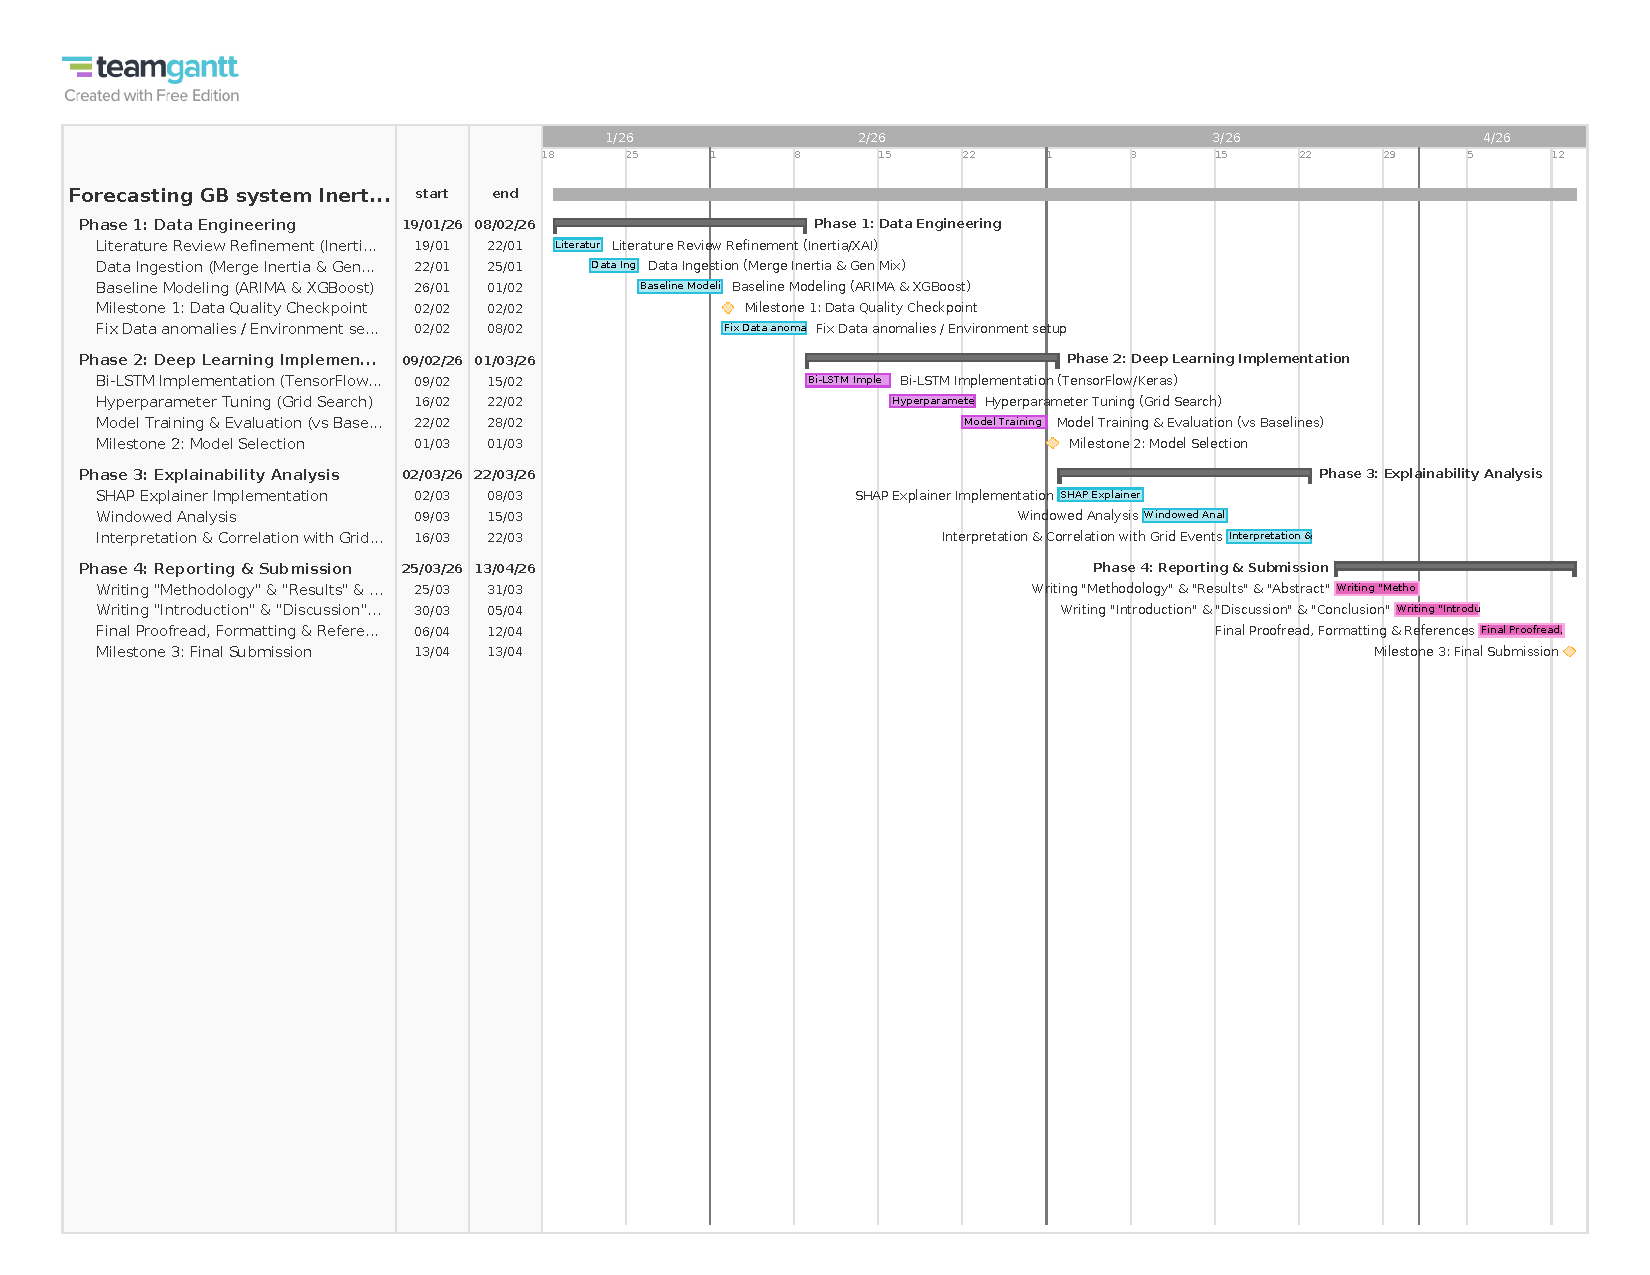
\includegraphics[page=1, width=0.8\textwidth]{Forecasting_GB_system_Inertia.pdf}
        \caption{Project Gantt chart depicts a 12-week timeline comprising 4 Phases and 3 Milestones.}
        \label{fig:my_gantt_chart}
    \end{figure}
\subsection{Deliverables}
This plan will deliver tangible output at each stage to ensure it meets the deadline.
\begin{itemize}
\item \textbf{Master Dataset (Week 1):} A fully preprocessed and time-aligned dataset, ready for modelling.
\item \textbf{Baseline Performance Evaluation (Week 2):} The RMSE/MAE comparison table, calculated using AARIMA and XGBoost, to determine the optimal score threshold for Bi-LSTM.
\item \textbf{Deep Learning Implementation (Week 4):} The full-fledged implementation of the Bi-LSTM network with a loss function.
\item \textbf{XAI Integration (Week 8):} SHAP integration with the best-performing model to produce the Summary and Force Plot.
\item \textbf{Final Dissertation (Week 12):} A complete dissertation report, which comprises the introduction, Literature Review, Methodology, Results, Discussion, and Conclusion.
\end{itemize}

\subsection{Milestones}
Each Milestone acts as a major decision point which dictates the project's direction.
\begin{itemize}
\item \textbf{Data Quality Checkpoint (Week 2):} If XGBoost accuracy is lower than expected in this milestone, then modelling will be paused to improve the data pipeline during week 3. Otherwise, the project will go as planned.
\item \textbf{Model Selection (Week 6):} If the Bi-LSTM is computationally heavy or underperforms, the XGBoost will be selected for Explainability Analysis.
\item \textbf{Dissertation Submission (Week 12):} Making everything ready for final submission, including the PDF report and GitHub code repository.
\end{itemize}


\printbibliography

\end{document}